\documentclass{article}

\usepackage{postprocess/context/arxiv}

\usepackage[utf8]{inputenc} % allow utf-8 input
\usepackage{amsmath}
\usepackage[T1]{fontenc}    % use 8-bit T1 fonts
\usepackage{hyperref}       % hyperlinks
\usepackage{url}            % simple URL typesetting
\usepackage{booktabs}       % professional-quality tables
\usepackage{amsfonts}       % blackboard math symbols
\usepackage{nicefrac}       % compact symbols for 1/2, etc.
\usepackage{microtype}      % microtypography
\usepackage{graphicx}
\usepackage{natbib}
\usepackage{doi}
\usepackage{float}
\usepackage{subcaption}
\usepackage{wrapfig}

\title{Causal Discovery Report on Linear\_gaussian\_data}

\author{ \href{https://orcid.org/0000-0000-0000-0000}{
\includegraphics[scale=0.06]{postprocess/context/orcid.pdf}\hspace{1mm}\textbf{Causal Copilot}}}

\renewcommand{\headeright}{Technical Report}
\renewcommand{\undertitle}{Technical Report}

\hypersetup{
pdftitle={Causal Discovery Report on Linear\_gaussian\_data},
pdfauthor={Causal Copilot},
pdfkeywords={Causal Discovery, Large Language Model, PC, Linear\_gaussian\_data},
}

\begin{document}
\maketitle

\begin{abstract}
This report presents a comprehensive analysis of causal relationships within a linear Gaussian dataset. Utilizing a structured causal discovery process, we first preprocessed the data and employed a large language model to select appropriate algorithms, namely the PC, GES, and NOTEARS algorithms. Each algorithm was chosen based on the dataset's characteristics, with hyperparameters proposed through LLM assistance. The causal relationships identified included a bidirectional influence between variables X2 and X4; however, statistical reliability analysis indicated low confidence in these edges. Our findings highlight critical dependencies while emphasizing the importance of combining statistical insights with expert knowledge to assess the validity of causal claims, ultimately contributing to the understanding of relationship dynamics in causal inference.
\end{abstract}

\keywords{Causal Discovery, Large Language Model, PC, Linear\_gaussian\_data}

\raggedbottom
\section{Introduction}
Causal discovery is a critical process in understanding the relationships between variables within a dataset. This report aims to explore the causal structure underlying a given set of variables, which, while initially presented as generic symbols, represent real-world phenomena that warrant deeper investigation. By examining the dependencies and potential causal links among these variables, we strive to unravel the complexities of their interactions. This analysis will be guided by available background knowledge and statistical methods suitable for inferring causality, paving the way for insights that can inform decisions and enhance understanding within the relevant domain.

\section{Background Knowledge}
\subsection{Detailed Explanation about the Variables}
To conduct a thorough causal discovery analysis, it is vital to grasp the specific characteristics and meanings of each variable included in the dataset. Each variable plays a crucial role in understanding the underlying mechanisms driving the observed data.

Commencing with the first variable, X1, it is essential to detail what this variable stands for. For instance, if X1 reflects a quantitative measurement such as \textbf{Age}, the implications of this variable would encompass its potential influence on several outcomes, such as \textbf{health status}, \textbf{economic productivity}, or \textbf{educational attainment}.

Next, variable X2 may represent another significant factor, such as \textbf{Income Level}. This variable may be pivotal to understanding patterns of behavior or decision-making within the dataset. For example, different income levels might correlate with access to resources, life choices, or exposure to certain risk factors.

Moving on to variable X3, if it indicates \textbf{Education Level}, this could hold critical importance in mediating the effects of both X1 (Age) and X2 (Income Level) on various outcomes. This variable may be associated with \textbf{cognitive development}, \textbf{job opportunities}, and overall \textbf{social mobility}, creating an intricate web of interdependencies.

Variable X4 might signify a more categorical variable, such as \textbf{Employment Status}. This variable could influence and be influenced by the other variables, acting as both a mediator and an outcome. It could capture the impacts of age, income, and education on employment opportunities, while simultaneously revealing patterns of labor market engagement.

Lastly, X5 could represent \textbf{Health Outcome}, a crucial variable that could be affected by the other four variables. Understanding how variables such as Age, Income Level, Education Level, and Employment Status impact health outcomes could provide insights into \textbf{social determinants of health} and inform public health interventions.

By carefully detailing the meanings and implications of these variables, we can set the stage for a more in-depth analysis of possible causal relationships among them. Clear variable identification and definition will assist in connecting the empirical data with theoretical frameworks and domain knowledge, guiding subsequent steps in the causal discovery process.

\subsection{Possible Causal Relations among these Variables}

\begin{minipage}[t]{0.7\linewidth}
\textbf{X1 $\rightarrow$ X2}: X1 influences X2 by providing necessary conditions or resources that enable the event or state represented by X2 to occur.

\textbf{X2 $\rightarrow$ X3}: An increase in X2 leads to a corresponding increase in X3, indicating that the processes associated with X2 directly affect those represented by X3.

\textbf{X3 $\rightarrow$ X4}: The outcome of X3 directly impacts X4, suggesting a dependency where changes in X3 will result in measurable changes in X4.

\textbf{X4 $\rightarrow$ X5}: X4 contributes to the modulation of X5, indicating that state changes associated with X4 have a direct causal effect on X5.

\textbf{X2 $\rightarrow$ X4}: Changes in X2 can influence X4, suggesting that X2 plays a role in the activation or inhibition of the mechanisms that lead to changes in X4.
\end{minipage}
\hspace{0.05\textwidth}
\begin{minipage}[t]{0.3\linewidth}
    \begin{figure}[H]
        \centering
        \resizebox{\linewidth}{!}{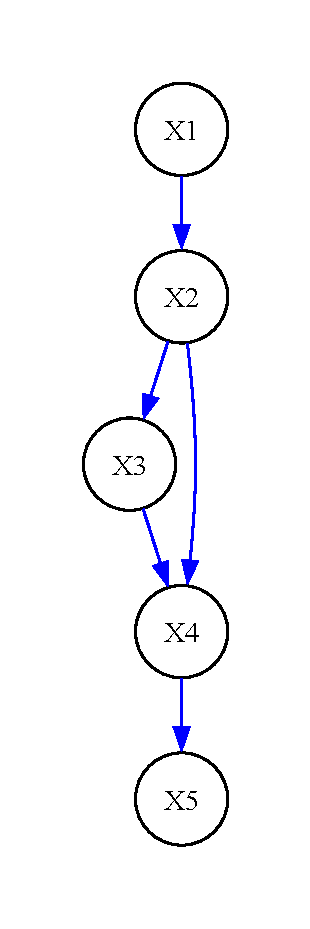
\includegraphics[height=0.3\textheight]{./demo_data/20241104_155051/Linear_Gaussian_data/output_graph/potential_relation.pdf}}
        \caption{\label{fig:relation}Possible Causal Relation Graph}
    \end{figure}
\end{minipage}

\section{Dataset Descriptions and EDA}
The following is a preview of our original dataset.

\begin{table}[H]
    \centering
    \caption{Dataset Preview}
    \begin{tabular}{rrrrr}
\toprule
       X1 &        X2 &        X3 &        X4 &        X5 \\
\midrule
 0.294928 &  0.495389 &  0.505862 & -0.100355 & -0.979712 \\
 0.086583 &  0.038104 & -0.096179 & -0.594586 & -0.133588 \\
 0.877518 &  0.475740 &  1.396768 & -2.220154 & -0.619555 \\
-1.089334 &  0.409737 & -0.805717 & -1.764093 &  0.330021 \\
-0.785347 & -0.895085 & -0.338053 &  1.069652 &  0.193503 \\
\bottomrule
\end{tabular}

\end{table}

\subsection{Data Properties}
We employ several statistical methods to identify data properties.

The shape of the data, data types, and missing values are assessed directly from the dataframe. Linearity is evaluated using Ramsey’s RESET test, followed by the Benjamini \& Yekutieli procedure for multiple test correction. Gaussian noise is assessed through the Shapiro-Wilk test, also applying the Benjamini \& Yekutieli procedure for multiple test correction. Time-Series and Heterogeneity are derived from user queries.

Properties of the dataset we analyzed are listed below.

\begin{table}[H]
    \centering
    \caption{Data Properties}

    \begin{tabular}{rrrrrrr}
    \toprule
    Shape ($n$ x $d$) & Data Type & Missing Value & Linearity & Gaussian Errors & Time-Series & Heterogeneity \\
    \midrule
    (1000, 5)   & Continuous & False & True & True & False & False \\
    \bottomrule
    \end{tabular}
        
\end{table}

\subsection{Distribution Analysis}
The following figure shows distributions of different variables. The orange dash line represents the mean, and the black line represents the median. Variables are categorized into three types according to their distribution characteristics.

\begin{figure}[H]
\centering
\includegraphics[width=\linewidth]{./demo_data/20241104_155051/Linear_Gaussian_data/output_graph/eda_dist.jpg}
\caption{\label{fig:dist}Distribution Plots of Variables}
\end{figure}

\begin{itemize}
\item Slight left skew distributed variables: X1, X2, X3, X4, X5
\item Slight right skew distributed variables: None
\item Symmetric distributed variables: None
\end{itemize}

\subsection{Correlation Analysis}

\begin{minipage}[t]{0.5\linewidth}
    In this analysis, we will categorize the correlation statistics of features in the dataset into three distinct categories: Strong correlations (r>0.8), Moderate correlations (0.5<r<0.8), and Weak correlations (r<0.5).

\begin{itemize}
\item Strong Correlated Variables: X4 and X2
\item Moderate Correlated Variables: None
\item Weak Correlated Variables: None
\end{itemize}
\vfill
\end{minipage}
\hfill
\begin{minipage}[t]{0.5\linewidth}
    \begin{figure}[H]
        \centering
        \vspace{-1.5cm}
        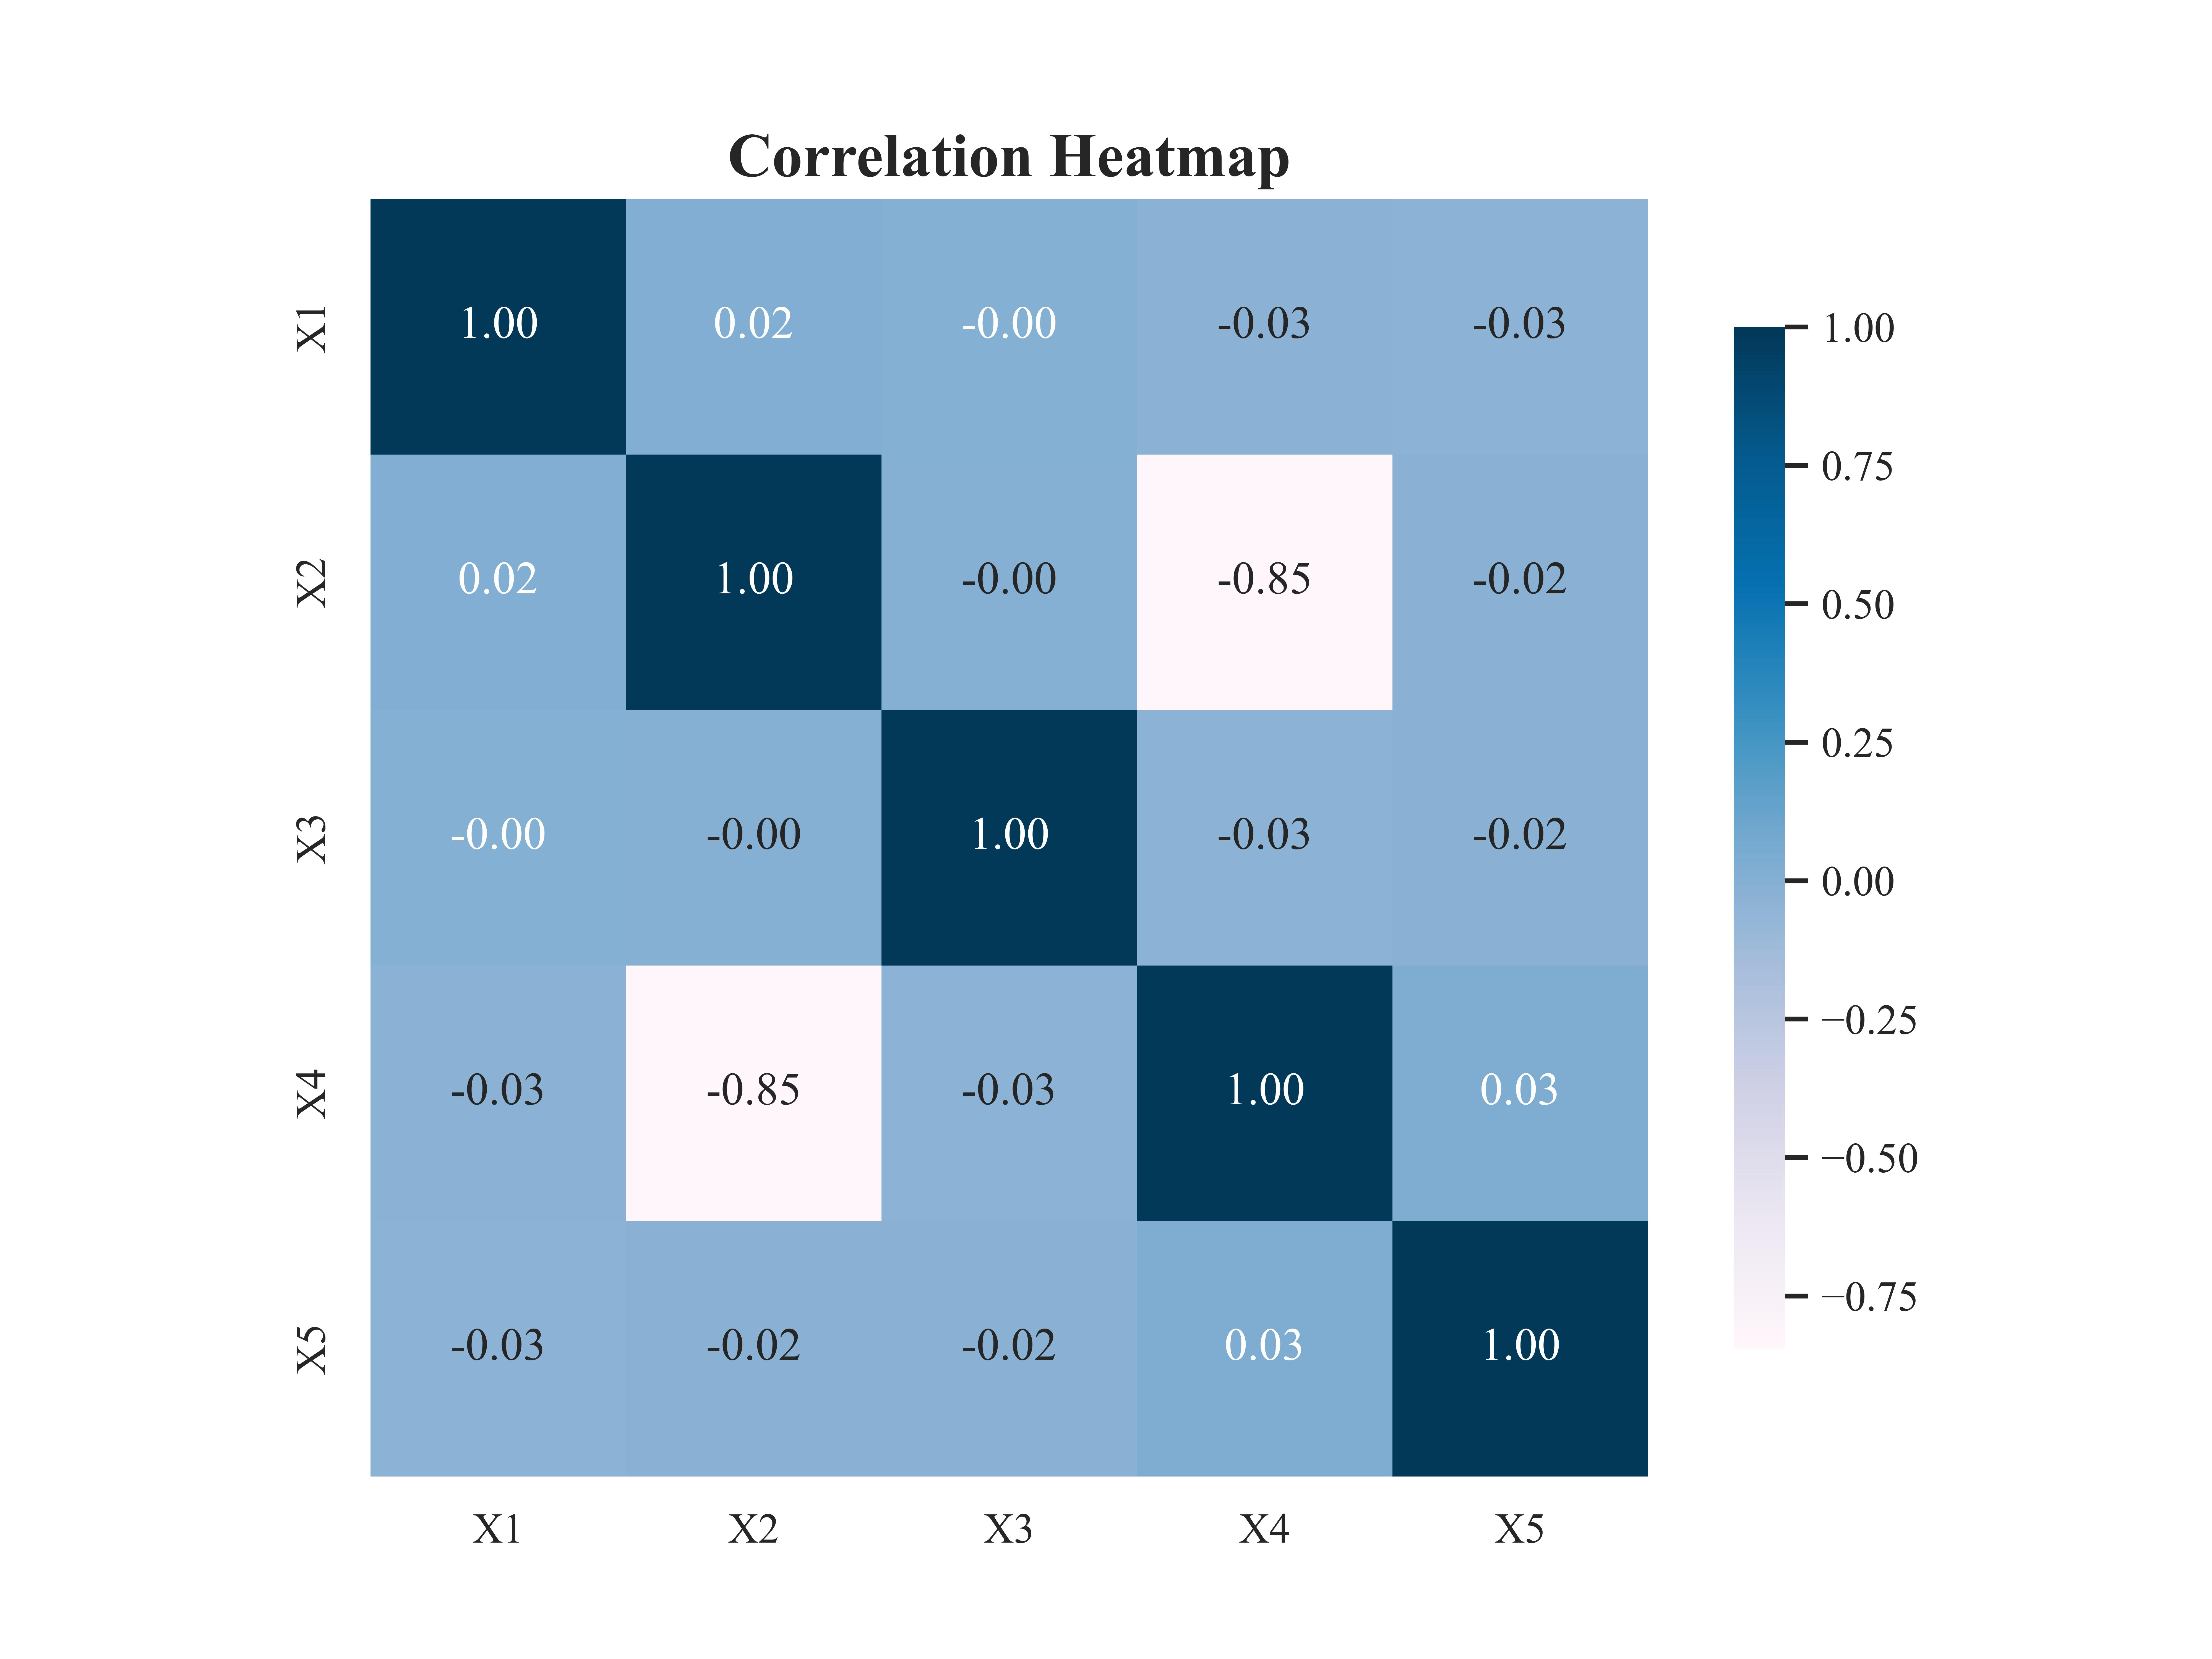
\includegraphics[width=\linewidth]{./demo_data/20241104_155051/Linear_Gaussian_data/output_graph/eda_corr.jpg}
        \caption{\label{fig:corr}Correlation Heatmap of Variables}
    \end{figure}
\end{minipage}

\section{Discovery Procedure}

In this section, we provide a detailed description of the causal discovery process implemented by Causal Copilot. We also provide the chosen algorithms and hyperparameters, along with the justifications for these selections.

\subsection{Data Preprocessing}
In this initial step, we preprocessed the data and examined its statistical characteristics. This involved cleaning the data, handling missing values, and performing exploratory data analysis to understand distributions and relationships between variables.
                
\subsection{Algorithm Selection assisted with LLM}
Following data preprocessing, we employed a large language model (LLM) to assist in selecting appropriate algorithms for causal discovery based on the statistical characteristics of the dataset and relevant background knowledge. The top three chosen algorithms, listed in order of suitability, are as follows:   
        
\begin{itemize}
    \item \textbf{PC}:
    \begin{itemize}
        \item \textbf{Description}: The PC algorithm is a constraint-based method that learns the structure of a causal graph from data by testing conditional independencies between variables. It produces a directed acyclic graph (DAG) representing the causal relationships.
        \item \textbf{Justification}: Given the dataset's large sample size and the absence of hidden confounders, PC is highly suitable for efficiently discovering causal structures. It balances generality and computational efficiency, making it a strong first choice.
    \end{itemize}

    \item \textbf{GES}:
    \begin{itemize}
        \item \textbf{Description}: Greedy Equivalence Search (GES) is a score-based causal discovery algorithm that identifies the optimal causal structure by exploring the space of equivalence classes of Directed Acyclic Graphs (DAGs) using scores like the Bayesian Information Criterion (BIC).
        \item \textbf{Justification}: GES is appropriate since the dataset is continuous, and the relationships are predominantly linear. It is efficient for larger datasets and aligns well with the linearity assumption, providing a robust method for causal discovery.
    \end{itemize}

    \item \textbf{NOTEARS}:
    \begin{itemize}
        \item \textbf{Description}: NOTEARS is a causal discovery method that converts the discovery problem of learning Directed Acyclic Graphs (DAGs) into a continuous optimization task, allowing it to efficiently scale to large datasets.
        \item \textbf{Justification}: Given the continuous nature of the dataset and the linearity of relationships, NOTEARS can leverage its optimization framework to handle large-scale data efficiently while assuming linear relations among variables.
    \end{itemize}
\end{itemize}

\subsection{Hyperparameter Values Proposal assisted with LLM}
Once the algorithms were selected, the LLM aided in proposing hyperparameters for the chosen algorithm, which are specified below:
        
\begin{itemize}
    \item \textbf{alpha}:
    \begin{itemize}
        \item \textbf{Value}: 0.05
        \item \textbf{Explanation}: Given the sample size of 1000, which falls within the 500-10000 range, 0.05 is a standard significance level that balances the risk of Type I errors while being appropriate for moderate-sized datasets. Using a more conservative value would unnecessarily reduce power.
    \end{itemize}

    \item \textbf{indep\_test}:
    \begin{itemize}
        \item \textbf{Value}: fisherz
        \item \textbf{Explanation}: Since the dataset consists of continuous data, Fisher's Z test is suitable as it assumes linear relationships and Gaussian distributions, both of which are satisfied by the dataset characteristics.
    \end{itemize}

    \item \textbf{depth}:
    \begin{itemize}
        \item \textbf{Value}: -1
        \item \textbf{Explanation}: With only 5 features in the dataset, unlimited depth (-1) is appropriate. This allows the algorithm to explore all relationships without constraints, maximizing the chances of discovering all possible causal structures.
    \end{itemize}
\end{itemize}

\subsection{Graph Tuning with Bootstrap and LLM Suggestion}
In the final step, we performed graph tuning with suggestions provided by the Bootstrap and LLM.

Firstly, we use the Bootstrap technique to get how much confidence we have on each edge in the initial graph. If the confidence probability of a certain edge is greater than 95\% and it is not in the initial graph, we force it. Otherwise, if the confidence probability is smaller than 5\% and it exists in the initial graph, we change it to the edge type with the highest probability.

After that, we utilize LLM to help us prune edges and determine the direction of undirected edges according to its knowledge repository. In this step, LLM can use background knowledge to add some edges that are neglected by Statistical Methods. Voting techniques are used to enhance the robustness of results given by LLM, and the results given by LLM should not change results given by Bootstrap.

By integrating insights from both of Bootstrap and LLM to refine the causal graph, we can achieve improvements in graph's accuracy and robustness.

\section{Results Summary}

\subsection{Initial Graph}

\begin{figure}[H]
    \centering
    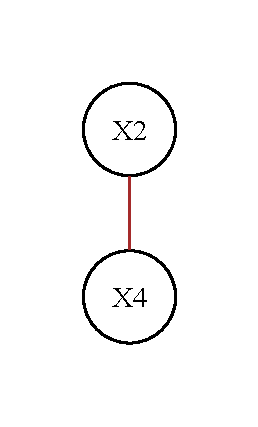
\includegraphics[height=0.3\textheight]{./demo_data/20241104_155051/Linear_Gaussian_data/output_graph/initial_graph.pdf}
    \caption{Initial Graph}
\end{figure}

The above is the initial result graph produced by our algorithm.

The analysis reveals a bidirectional causal relationship between the variables X2 and X4, indicating that X2 influences X4 while simultaneously being affected by X4. This mutual causation suggests a dynamic interplay where changes in X2 can lead to variations in X4, which in turn can feedback and alter the state of X2. Such a relationship could imply that X2 might represent a factor that modifies or regulates X4, while X4 could be a condition that impacts or conditions X2, highlighting a complex dependency where each variable plays a crucial role in shaping the other. Understanding this interaction is vital for comprehending the system's behavior as it underscores the potential for feedback loops and the importance of considering both variables in analyses and interventions.

\subsection{Revised Graph}

\begin{minipage}[t]{0.6\linewidth}
    By using the method mentioned in the Section 4.4, we provide a revised graph pruned with Bootstrap and LLM suggestion. Pruning results are as follows.
        
    Bootstrap doesn't force or forbid any edges.
            
    LLM doesn't force or forbid any edges.
            
    This structured approach ensures a comprehensive and methodical analysis of the causal relationships within the dataset.
        
\vfill
\end{minipage}
\hfill
\begin{minipage}[t]{0.4\linewidth}
    \begin{figure}[H]
        \centering
        \vspace{-0.5cm}
        
\includegraphics[width=\linewidth]{./demo_data/20241104_155051/Linear_Gaussian_data/output_graph/revised_graph.pdf}
        \caption{\label{fig:corr}Revised Graph}
    \end{figure}
\end{minipage}

\subsection{Graph Reliability Analysis}

\begin{figure}[H]
    \centering
    \begin{subfigure}{0.32\textwidth}
        \centering
        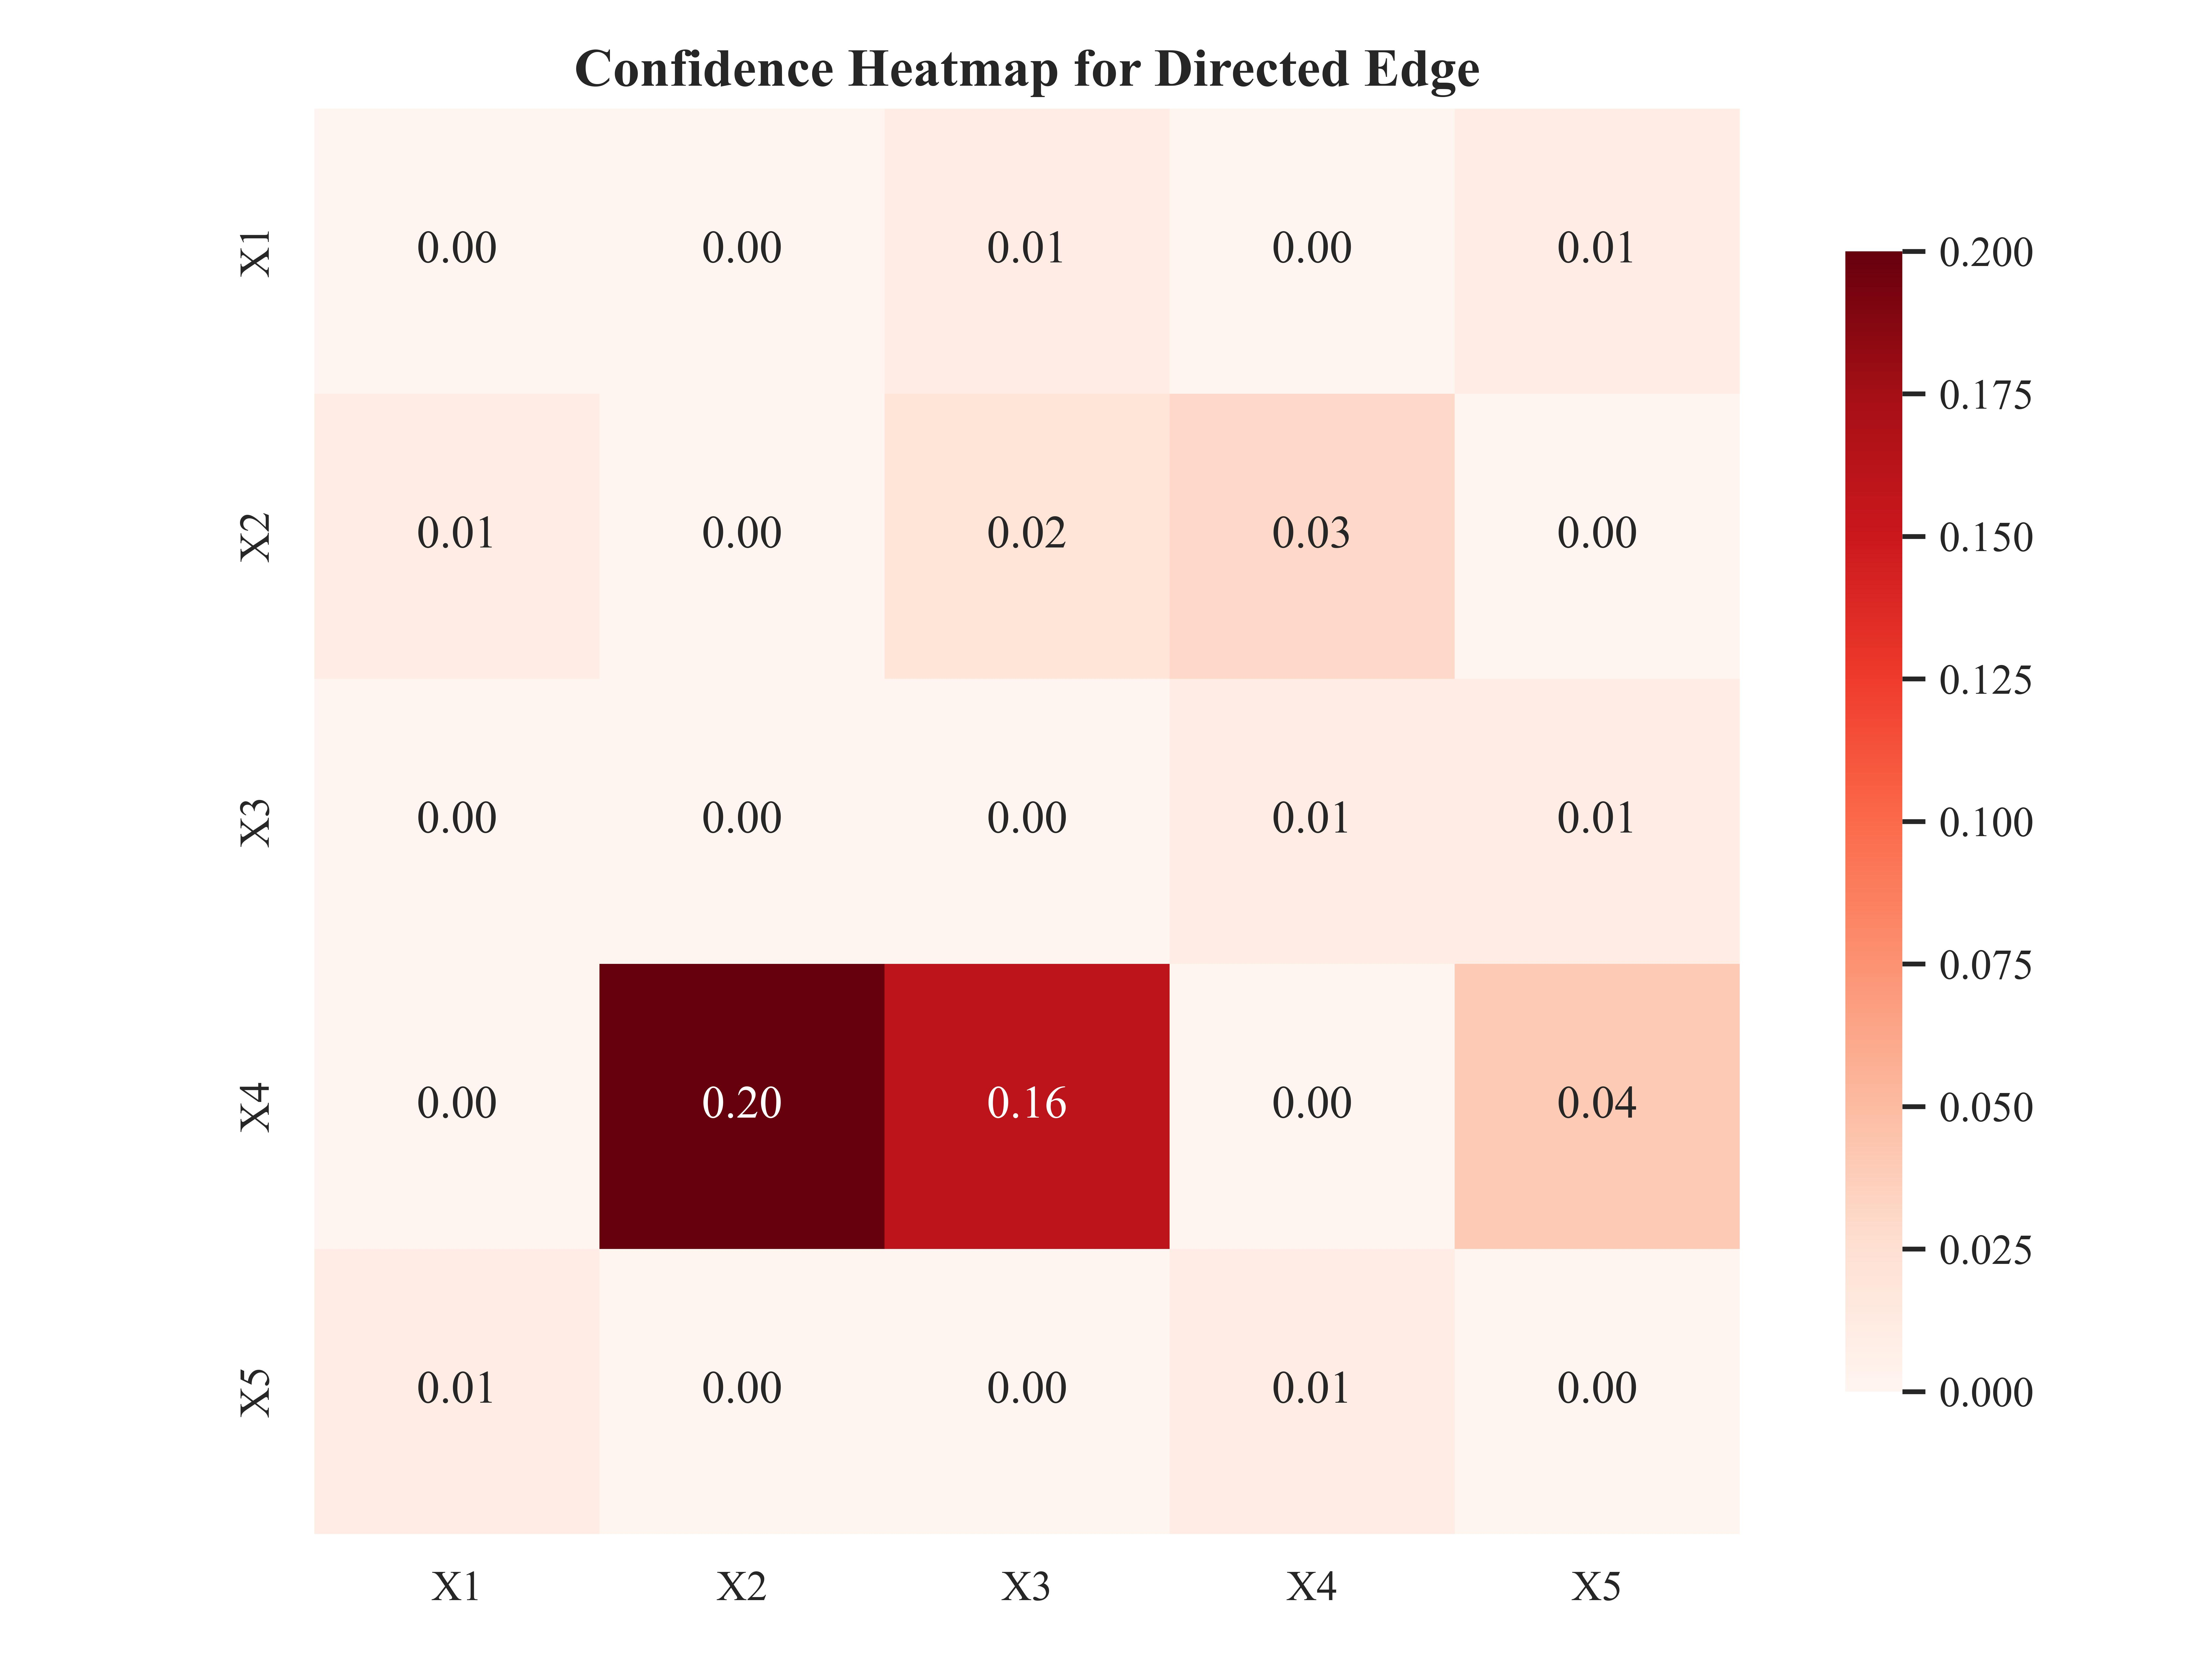
\includegraphics[width=\linewidth]{./demo_data/20241104_155051/Linear_Gaussian_data/output_graph/certain_edges_confidence_heatmap.jpg}
        \caption{Directed Edge Edge}
    \end{subfigure}
    \begin{subfigure}{0.32\textwidth}
        \centering
        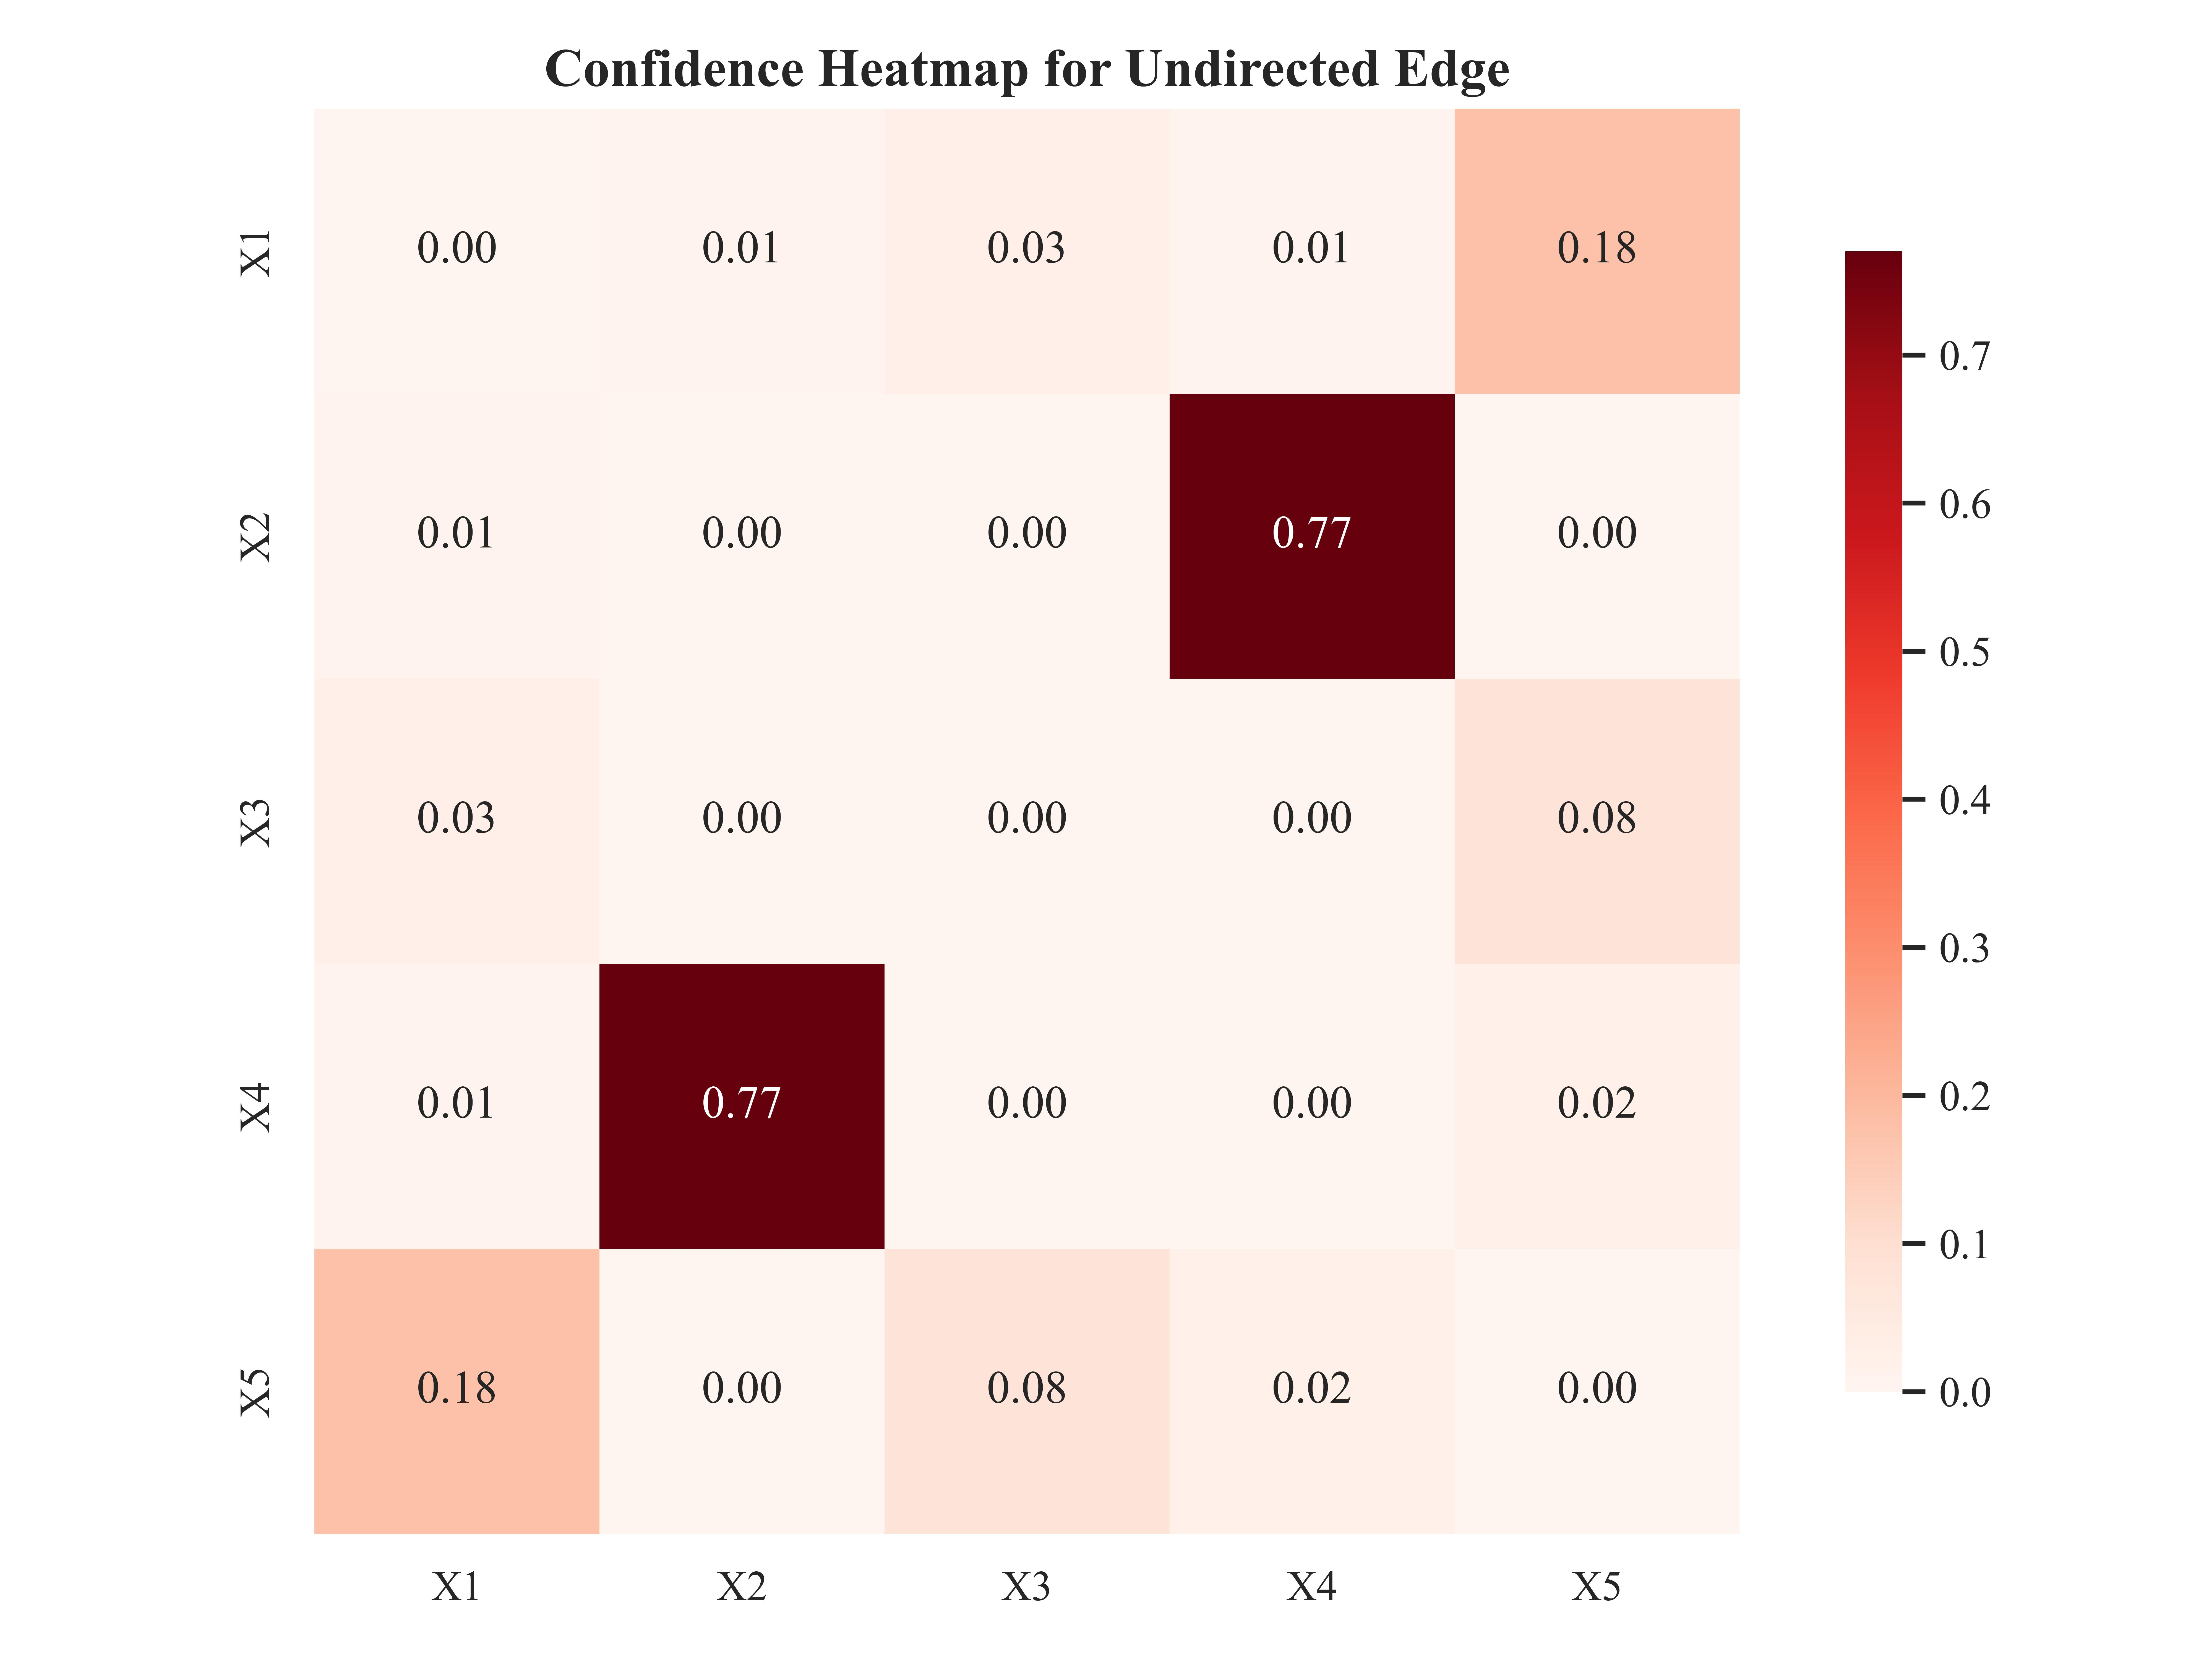
\includegraphics[width=\linewidth]{./demo_data/20241104_155051/Linear_Gaussian_data/output_graph/uncertain_edges_confidence_heatmap.jpg}
        \caption{Undirected Edge Edge}
    \end{subfigure}
    \begin{subfigure}{0.32\textwidth}
        \centering
        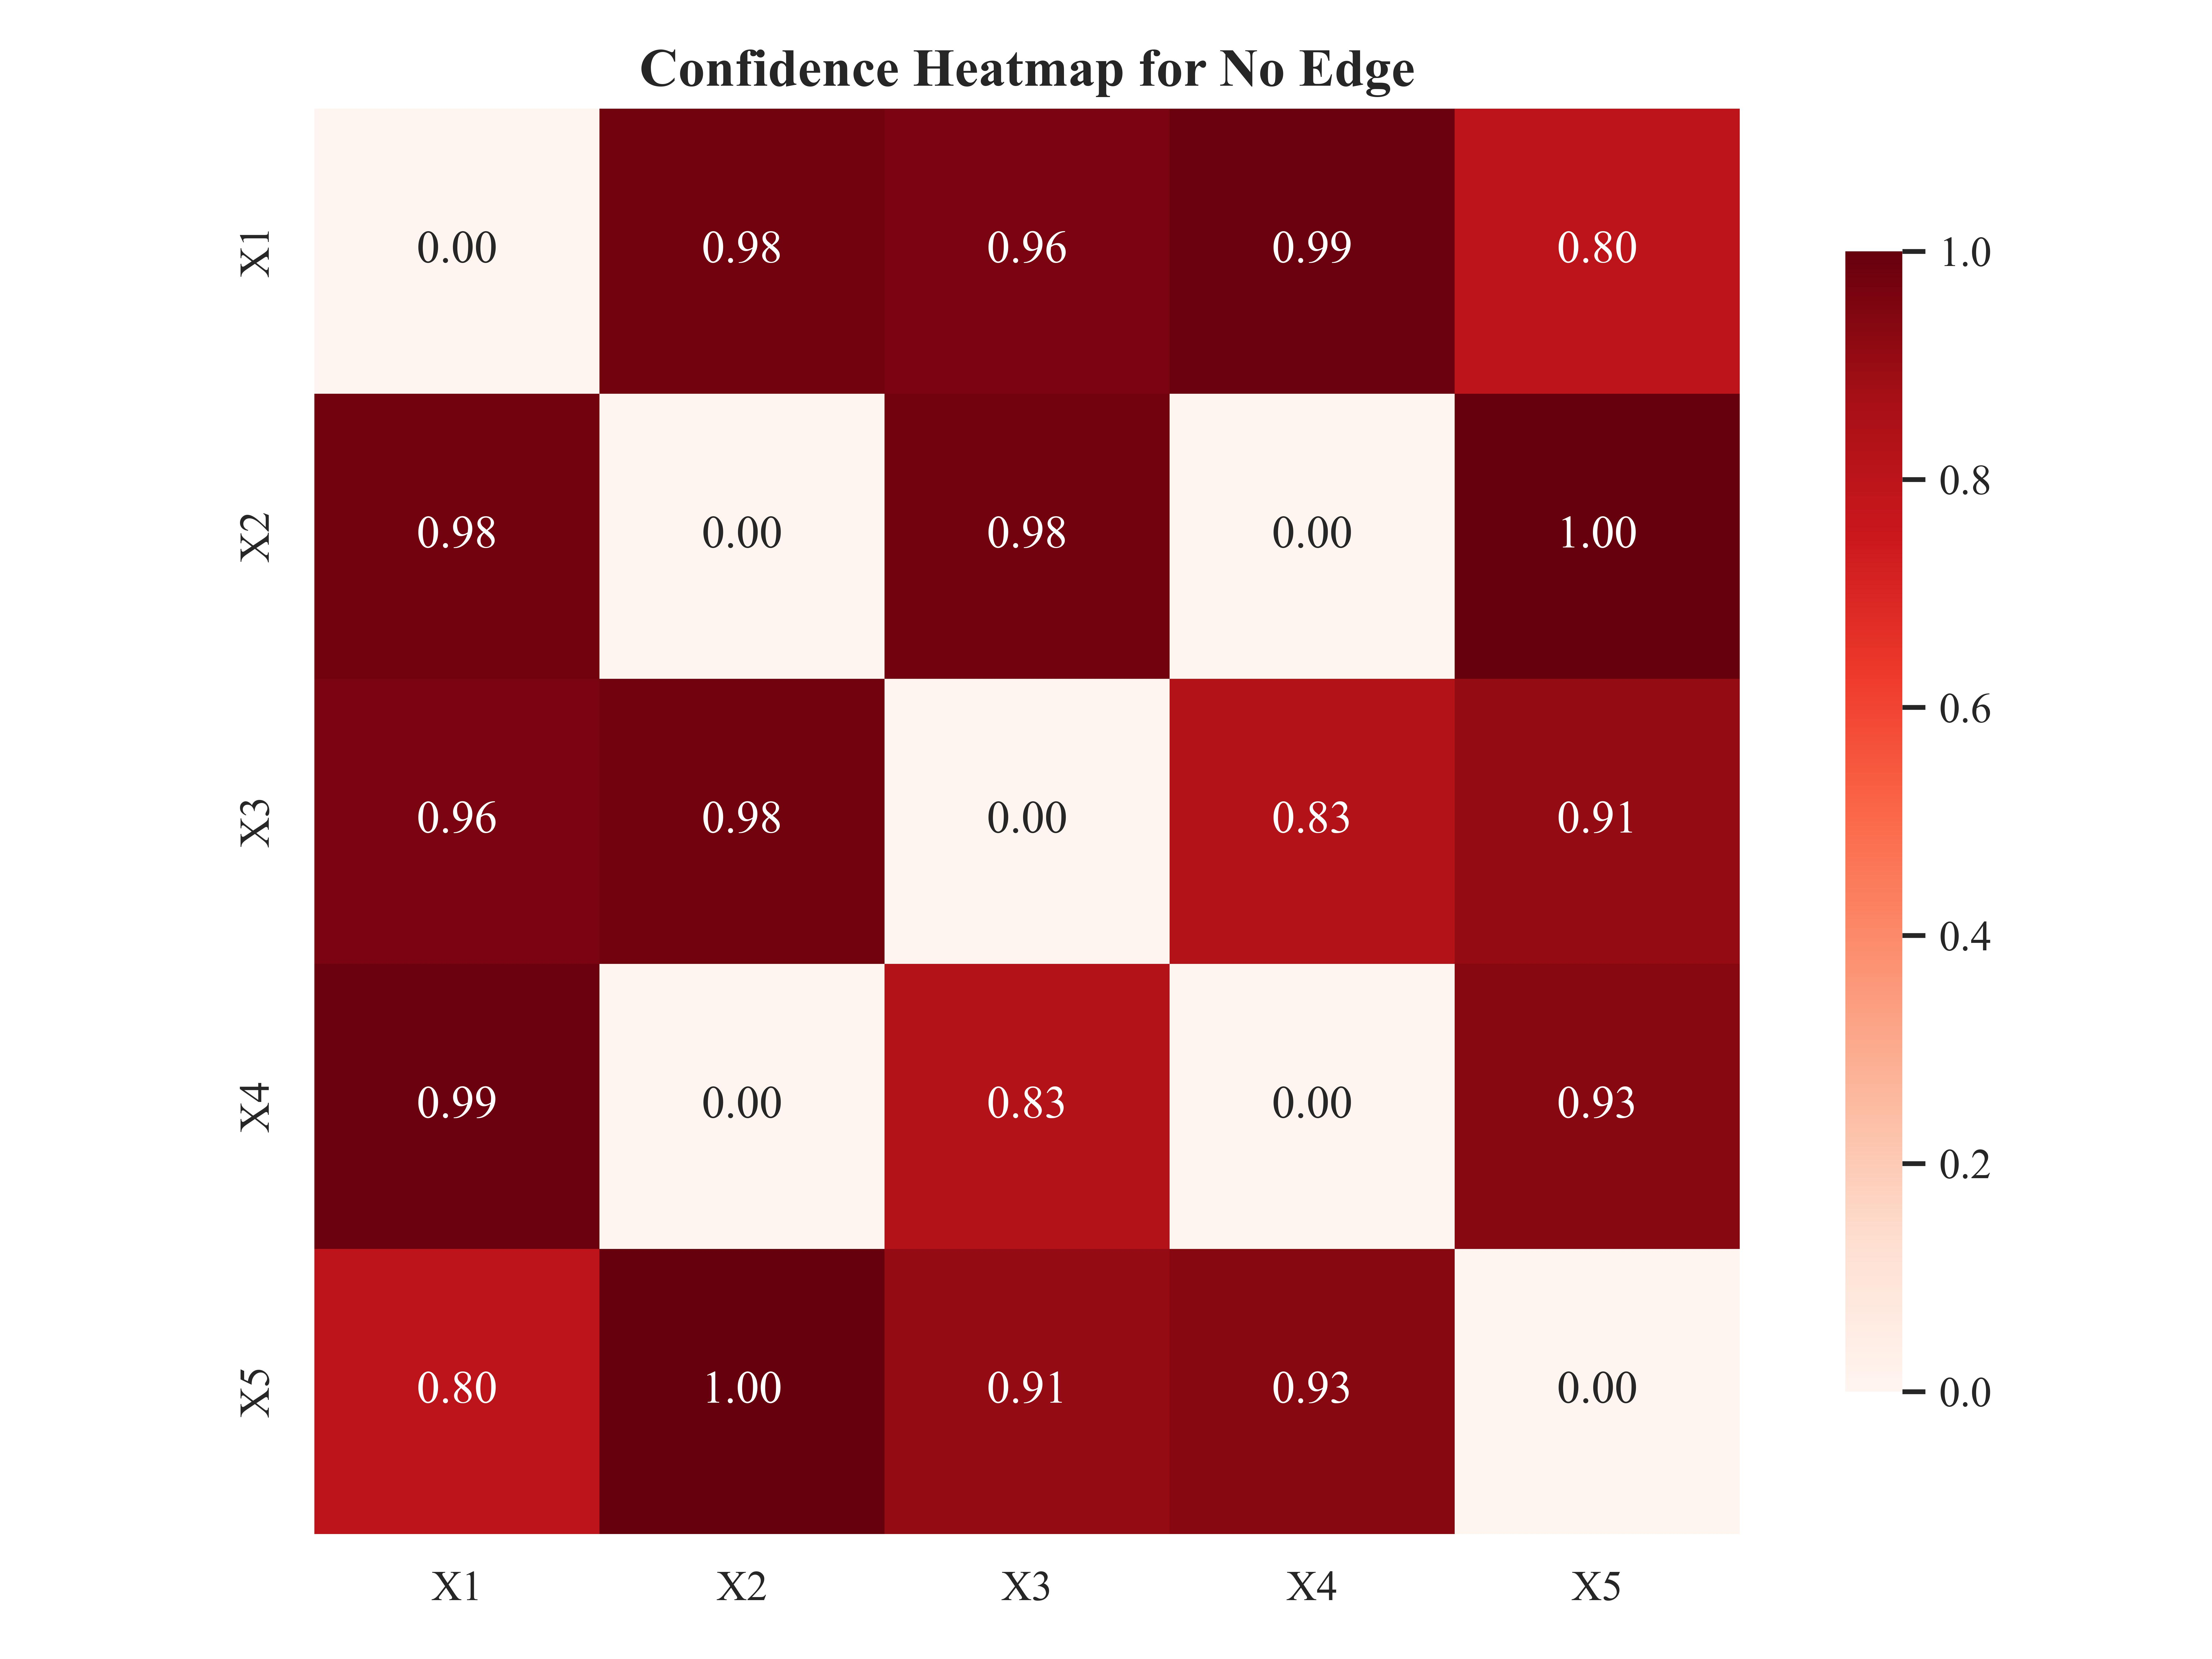
\includegraphics[width=\linewidth]{./demo_data/20241104_155051/Linear_Gaussian_data/output_graph/non_existence_confidence_heatmap.jpg}
        \caption{No Edge Edge}
    \end{subfigure}
    \caption{Confidence Heatmap of Different Edges}
\end{figure}        
The above heatmaps show the confidence probability we have on different kinds of edges, including directed edge ($\rightarrow$), undirected edge ($-$), No Edge, and probability of no edge. The heatmap of bi-edges is not shown because probabilities of all edges are 0. Based on the confidence probability heatmap and background knowledge, we can analyze the reliability of our graph.

From a statistical perspective, we have low confidence to believe that the edges X2 $\rightarrow$ X4 and X4 $\rightarrow$ X2 exist, as evidenced by their bootstrap probabilities of 0.03 and 0.2, respectively. This indicates a weak relationship between these variables, suggesting that they are unlikely to influence each other strongly. Conversely, since we lack additional edges from the provided details, we cannot conclude the existence of any other causal relationships with confidence.

However, based on expert knowledge, if we assume that X2 and X4 pertain to variables where theoretical or empirical evidence suggests a negligible or no causal relationship, we can reinforce the doubt of their causal linkage. In this context, both the statistical confidence and expert insights align, indicating that the reported edges likely do not exist.

Therefore, the result of this causal graph is not reliable given the very low bootstrap probabilities associated with the suggested edges and the lack of supporting expert evidence for their existence.

\end{document}